% Created by tikzDevice version 0.12.6 on 2024-04-11 10:03:55
% !TEX encoding = UTF-8 Unicode
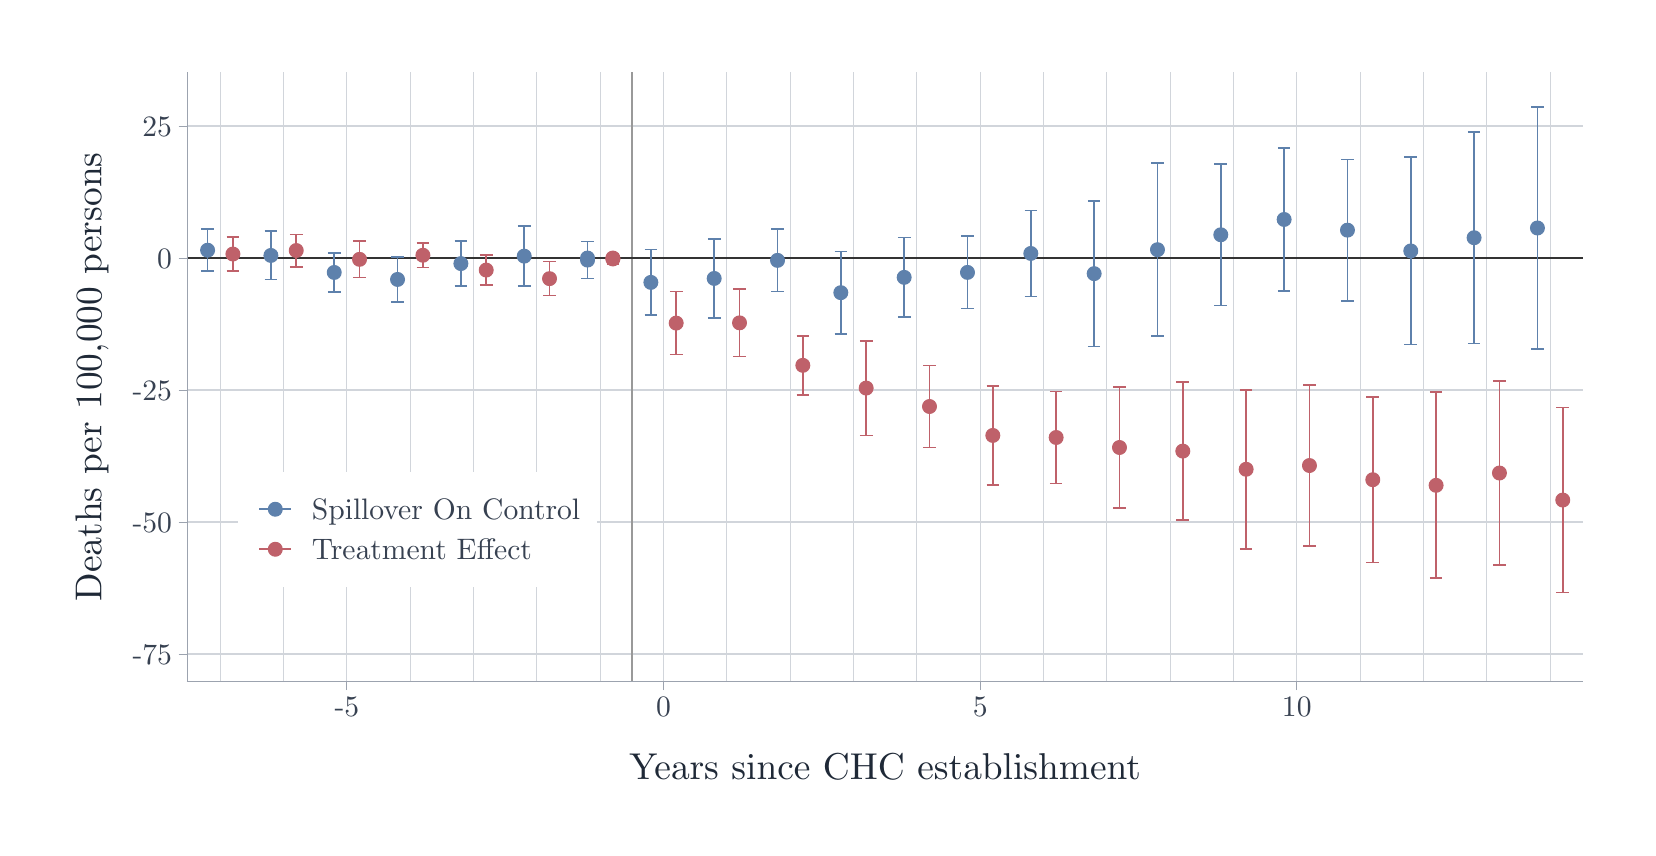
\begin{tikzpicture}[x=1pt,y=1pt]
\definecolor{fillColor}{RGB}{255,255,255}
\path[use as bounding box,fill=fillColor] (0,0) rectangle (578.16,289.08);
\begin{scope}
\path[clip] (  0.00,  0.00) rectangle (578.16,289.08);
\definecolor{drawColor}{RGB}{255,255,255}

\path[draw=drawColor,line width= 0.6pt,line join=round,line cap=round,fill=fillColor] ( -0.00,  0.00) rectangle (578.16,289.08);
\end{scope}
\begin{scope}
\path[clip] ( 57.55, 52.74) rectangle (562.16,273.08);
\definecolor{drawColor}{RGB}{255,255,255}
\definecolor{fillColor}{RGB}{255,255,255}

\path[draw=drawColor,line width= 0.6pt,line join=round,line cap=round,fill=fillColor] ( 57.55, 52.74) rectangle (562.16,273.08);
\definecolor{drawColor}{RGB}{209,213,219}

\path[draw=drawColor,line width= 0.4pt,line join=round] ( 69.58, 52.74) --
	( 69.58,273.08);

\path[draw=drawColor,line width= 0.4pt,line join=round] ( 92.46, 52.74) --
	( 92.46,273.08);

\path[draw=drawColor,line width= 0.4pt,line join=round] (138.23, 52.74) --
	(138.23,273.08);

\path[draw=drawColor,line width= 0.4pt,line join=round] (161.11, 52.74) --
	(161.11,273.08);

\path[draw=drawColor,line width= 0.4pt,line join=round] (184.00, 52.74) --
	(184.00,273.08);

\path[draw=drawColor,line width= 0.4pt,line join=round] (206.88, 52.74) --
	(206.88,273.08);

\path[draw=drawColor,line width= 0.4pt,line join=round] (252.65, 52.74) --
	(252.65,273.08);

\path[draw=drawColor,line width= 0.4pt,line join=round] (275.53, 52.74) --
	(275.53,273.08);

\path[draw=drawColor,line width= 0.4pt,line join=round] (298.41, 52.74) --
	(298.41,273.08);

\path[draw=drawColor,line width= 0.4pt,line join=round] (321.29, 52.74) --
	(321.29,273.08);

\path[draw=drawColor,line width= 0.4pt,line join=round] (367.06, 52.74) --
	(367.06,273.08);

\path[draw=drawColor,line width= 0.4pt,line join=round] (389.94, 52.74) --
	(389.94,273.08);

\path[draw=drawColor,line width= 0.4pt,line join=round] (412.83, 52.74) --
	(412.83,273.08);

\path[draw=drawColor,line width= 0.4pt,line join=round] (435.71, 52.74) --
	(435.71,273.08);

\path[draw=drawColor,line width= 0.4pt,line join=round] (481.47, 52.74) --
	(481.47,273.08);

\path[draw=drawColor,line width= 0.4pt,line join=round] (504.36, 52.74) --
	(504.36,273.08);

\path[draw=drawColor,line width= 0.4pt,line join=round] (527.24, 52.74) --
	(527.24,273.08);

\path[draw=drawColor,line width= 0.4pt,line join=round] (550.12, 52.74) --
	(550.12,273.08);

\path[draw=drawColor,line width= 0.4pt,line join=round] ( 57.55, 62.76) --
	(562.16, 62.76);

\path[draw=drawColor,line width= 0.4pt,line join=round] ( 57.55,110.45) --
	(562.16,110.45);

\path[draw=drawColor,line width= 0.4pt,line join=round] ( 57.55,158.14) --
	(562.16,158.14);

\path[draw=drawColor,line width= 0.4pt,line join=round] ( 57.55,205.83) --
	(562.16,205.83);

\path[draw=drawColor,line width= 0.4pt,line join=round] ( 57.55,253.53) --
	(562.16,253.53);

\path[draw=drawColor,line width= 0.4pt,line join=round] (115.35, 52.74) --
	(115.35,273.08);

\path[draw=drawColor,line width= 0.4pt,line join=round] (229.76, 52.74) --
	(229.76,273.08);

\path[draw=drawColor,line width= 0.4pt,line join=round] (344.18, 52.74) --
	(344.18,273.08);

\path[draw=drawColor,line width= 0.4pt,line join=round] (458.59, 52.74) --
	(458.59,273.08);
\definecolor{drawColor}{gray}{0.60}

\path[draw=drawColor,line width= 0.6pt,line join=round] (218.32, 52.74) -- (218.32,273.08);
\definecolor{drawColor}{gray}{0.20}

\path[draw=drawColor,line width= 0.6pt,line join=round] ( 57.55,205.83) -- (562.16,205.83);
\definecolor{drawColor}{RGB}{191,97,106}
\definecolor{fillColor}{RGB}{191,97,106}

\path[draw=drawColor,line width= 0.4pt,line join=round,line cap=round,fill=fillColor] ( 74.16,207.28) circle (  2.50);

\path[draw=drawColor,line width= 0.4pt,line join=round,line cap=round,fill=fillColor] ( 97.04,208.55) circle (  2.50);

\path[draw=drawColor,line width= 0.4pt,line join=round,line cap=round,fill=fillColor] (119.92,205.36) circle (  2.50);

\path[draw=drawColor,line width= 0.4pt,line join=round,line cap=round,fill=fillColor] (142.81,206.84) circle (  2.50);

\path[draw=drawColor,line width= 0.4pt,line join=round,line cap=round,fill=fillColor] (165.69,201.49) circle (  2.50);

\path[draw=drawColor,line width= 0.4pt,line join=round,line cap=round,fill=fillColor] (188.57,198.39) circle (  2.50);

\path[draw=drawColor,line width= 0.4pt,line join=round,line cap=round,fill=fillColor] (211.46,205.49) circle (  2.50);

\path[draw=drawColor,line width= 0.4pt,line join=round,line cap=round,fill=fillColor] (234.34,182.33) circle (  2.50);

\path[draw=drawColor,line width= 0.4pt,line join=round,line cap=round,fill=fillColor] (257.22,182.42) circle (  2.50);

\path[draw=drawColor,line width= 0.4pt,line join=round,line cap=round,fill=fillColor] (280.10,167.06) circle (  2.50);

\path[draw=drawColor,line width= 0.4pt,line join=round,line cap=round,fill=fillColor] (302.99,158.85) circle (  2.50);

\path[draw=drawColor,line width= 0.4pt,line join=round,line cap=round,fill=fillColor] (325.87,152.19) circle (  2.50);

\path[draw=drawColor,line width= 0.4pt,line join=round,line cap=round,fill=fillColor] (348.75,141.73) circle (  2.50);

\path[draw=drawColor,line width= 0.4pt,line join=round,line cap=round,fill=fillColor] (371.64,140.99) circle (  2.50);

\path[draw=drawColor,line width= 0.4pt,line join=round,line cap=round,fill=fillColor] (394.52,137.38) circle (  2.50);

\path[draw=drawColor,line width= 0.4pt,line join=round,line cap=round,fill=fillColor] (417.40,136.07) circle (  2.50);

\path[draw=drawColor,line width= 0.4pt,line join=round,line cap=round,fill=fillColor] (440.29,129.50) circle (  2.50);

\path[draw=drawColor,line width= 0.4pt,line join=round,line cap=round,fill=fillColor] (463.17,130.86) circle (  2.50);

\path[draw=drawColor,line width= 0.4pt,line join=round,line cap=round,fill=fillColor] (486.05,125.73) circle (  2.50);

\path[draw=drawColor,line width= 0.4pt,line join=round,line cap=round,fill=fillColor] (508.93,123.70) circle (  2.50);

\path[draw=drawColor,line width= 0.4pt,line join=round,line cap=round,fill=fillColor] (531.82,128.15) circle (  2.50);

\path[draw=drawColor,line width= 0.4pt,line join=round,line cap=round,fill=fillColor] (554.70,118.39) circle (  2.50);
\definecolor{drawColor}{RGB}{94,129,172}
\definecolor{fillColor}{RGB}{94,129,172}

\path[draw=drawColor,line width= 0.4pt,line join=round,line cap=round,fill=fillColor] ( 65.01,208.66) circle (  2.50);

\path[draw=drawColor,line width= 0.4pt,line join=round,line cap=round,fill=fillColor] ( 87.89,206.77) circle (  2.50);

\path[draw=drawColor,line width= 0.4pt,line join=round,line cap=round,fill=fillColor] (110.77,200.63) circle (  2.50);

\path[draw=drawColor,line width= 0.4pt,line join=round,line cap=round,fill=fillColor] (133.65,198.10) circle (  2.50);

\path[draw=drawColor,line width= 0.4pt,line join=round,line cap=round,fill=fillColor] (156.54,203.83) circle (  2.50);

\path[draw=drawColor,line width= 0.4pt,line join=round,line cap=round,fill=fillColor] (179.42,206.52) circle (  2.50);

\path[draw=drawColor,line width= 0.4pt,line join=round,line cap=round,fill=fillColor] (202.30,205.09) circle (  2.50);

\path[draw=drawColor,line width= 0.4pt,line join=round,line cap=round,fill=fillColor] (225.19,197.03) circle (  2.50);

\path[draw=drawColor,line width= 0.4pt,line join=round,line cap=round,fill=fillColor] (248.07,198.46) circle (  2.50);

\path[draw=drawColor,line width= 0.4pt,line join=round,line cap=round,fill=fillColor] (270.95,204.99) circle (  2.50);

\path[draw=drawColor,line width= 0.4pt,line join=round,line cap=round,fill=fillColor] (293.83,193.32) circle (  2.50);

\path[draw=drawColor,line width= 0.4pt,line join=round,line cap=round,fill=fillColor] (316.72,198.85) circle (  2.50);

\path[draw=drawColor,line width= 0.4pt,line join=round,line cap=round,fill=fillColor] (339.60,200.64) circle (  2.50);

\path[draw=drawColor,line width= 0.4pt,line join=round,line cap=round,fill=fillColor] (362.48,207.49) circle (  2.50);

\path[draw=drawColor,line width= 0.4pt,line join=round,line cap=round,fill=fillColor] (385.37,200.20) circle (  2.50);

\path[draw=drawColor,line width= 0.4pt,line join=round,line cap=round,fill=fillColor] (408.25,208.84) circle (  2.50);

\path[draw=drawColor,line width= 0.4pt,line join=round,line cap=round,fill=fillColor] (431.13,214.24) circle (  2.50);

\path[draw=drawColor,line width= 0.4pt,line join=round,line cap=round,fill=fillColor] (454.02,219.77) circle (  2.50);

\path[draw=drawColor,line width= 0.4pt,line join=round,line cap=round,fill=fillColor] (476.90,215.91) circle (  2.50);

\path[draw=drawColor,line width= 0.4pt,line join=round,line cap=round,fill=fillColor] (499.78,208.40) circle (  2.50);

\path[draw=drawColor,line width= 0.4pt,line join=round,line cap=round,fill=fillColor] (522.66,213.18) circle (  2.50);

\path[draw=drawColor,line width= 0.4pt,line join=round,line cap=round,fill=fillColor] (545.55,216.69) circle (  2.50);

\path[draw=drawColor,line width= 0.4pt,line join=round,line cap=round,fill=fillColor] (202.30,205.83) circle (  2.50);
\definecolor{drawColor}{RGB}{191,97,106}
\definecolor{fillColor}{RGB}{191,97,106}

\path[draw=drawColor,line width= 0.4pt,line join=round,line cap=round,fill=fillColor] (211.46,205.83) circle (  2.50);

\path[draw=drawColor,line width= 0.6pt,line join=round] ( 71.87,213.35) --
	( 76.45,213.35);

\path[draw=drawColor,line width= 0.6pt,line join=round] ( 74.16,213.35) --
	( 74.16,201.22);

\path[draw=drawColor,line width= 0.6pt,line join=round] ( 71.87,201.22) --
	( 76.45,201.22);

\path[draw=drawColor,line width= 0.6pt,line join=round] ( 94.75,214.39) --
	( 99.33,214.39);

\path[draw=drawColor,line width= 0.6pt,line join=round] ( 97.04,214.39) --
	( 97.04,202.71);

\path[draw=drawColor,line width= 0.6pt,line join=round] ( 94.75,202.71) --
	( 99.33,202.71);

\path[draw=drawColor,line width= 0.6pt,line join=round] (117.64,211.93) --
	(122.21,211.93);

\path[draw=drawColor,line width= 0.6pt,line join=round] (119.92,211.93) --
	(119.92,198.79);

\path[draw=drawColor,line width= 0.6pt,line join=round] (117.64,198.79) --
	(122.21,198.79);

\path[draw=drawColor,line width= 0.6pt,line join=round] (140.52,211.26) --
	(145.10,211.26);

\path[draw=drawColor,line width= 0.6pt,line join=round] (142.81,211.26) --
	(142.81,202.42);

\path[draw=drawColor,line width= 0.6pt,line join=round] (140.52,202.42) --
	(145.10,202.42);

\path[draw=drawColor,line width= 0.6pt,line join=round] (163.40,206.93) --
	(167.98,206.93);

\path[draw=drawColor,line width= 0.6pt,line join=round] (165.69,206.93) --
	(165.69,196.06);

\path[draw=drawColor,line width= 0.6pt,line join=round] (163.40,196.06) --
	(167.98,196.06);

\path[draw=drawColor,line width= 0.6pt,line join=round] (186.28,204.53) --
	(190.86,204.53);

\path[draw=drawColor,line width= 0.6pt,line join=round] (188.57,204.53) --
	(188.57,192.25);

\path[draw=drawColor,line width= 0.6pt,line join=round] (186.28,192.25) --
	(190.86,192.25);

\path[draw=drawColor,line width= 0.6pt,line join=round] (209.17,207.32) --
	(213.74,207.32);

\path[draw=drawColor,line width= 0.6pt,line join=round] (211.46,207.32) --
	(211.46,203.65);

\path[draw=drawColor,line width= 0.6pt,line join=round] (209.17,203.65) --
	(213.74,203.65);

\path[draw=drawColor,line width= 0.6pt,line join=round] (232.05,193.74) --
	(236.63,193.74);

\path[draw=drawColor,line width= 0.6pt,line join=round] (234.34,193.74) --
	(234.34,170.93);

\path[draw=drawColor,line width= 0.6pt,line join=round] (232.05,170.93) --
	(236.63,170.93);

\path[draw=drawColor,line width= 0.6pt,line join=round] (254.93,194.64) --
	(259.51,194.64);

\path[draw=drawColor,line width= 0.6pt,line join=round] (257.22,194.64) --
	(257.22,170.21);

\path[draw=drawColor,line width= 0.6pt,line join=round] (254.93,170.21) --
	(259.51,170.21);

\path[draw=drawColor,line width= 0.6pt,line join=round] (277.82,177.73) --
	(282.39,177.73);

\path[draw=drawColor,line width= 0.6pt,line join=round] (280.10,177.73) --
	(280.10,156.38);

\path[draw=drawColor,line width= 0.6pt,line join=round] (277.82,156.38) --
	(282.39,156.38);

\path[draw=drawColor,line width= 0.6pt,line join=round] (300.70,175.96) --
	(305.28,175.96);

\path[draw=drawColor,line width= 0.6pt,line join=round] (302.99,175.96) --
	(302.99,141.73);

\path[draw=drawColor,line width= 0.6pt,line join=round] (300.70,141.73) --
	(305.28,141.73);

\path[draw=drawColor,line width= 0.6pt,line join=round] (323.58,167.04) --
	(328.16,167.04);

\path[draw=drawColor,line width= 0.6pt,line join=round] (325.87,167.04) --
	(325.87,137.34);

\path[draw=drawColor,line width= 0.6pt,line join=round] (323.58,137.34) --
	(328.16,137.34);

\path[draw=drawColor,line width= 0.6pt,line join=round] (346.47,159.68) --
	(351.04,159.68);

\path[draw=drawColor,line width= 0.6pt,line join=round] (348.75,159.68) --
	(348.75,123.79);

\path[draw=drawColor,line width= 0.6pt,line join=round] (346.47,123.79) --
	(351.04,123.79);

\path[draw=drawColor,line width= 0.6pt,line join=round] (369.35,157.59) --
	(373.92,157.59);

\path[draw=drawColor,line width= 0.6pt,line join=round] (371.64,157.59) --
	(371.64,124.40);

\path[draw=drawColor,line width= 0.6pt,line join=round] (369.35,124.40) --
	(373.92,124.40);

\path[draw=drawColor,line width= 0.6pt,line join=round] (392.23,159.29) --
	(396.81,159.29);

\path[draw=drawColor,line width= 0.6pt,line join=round] (394.52,159.29) --
	(394.52,115.48);

\path[draw=drawColor,line width= 0.6pt,line join=round] (392.23,115.48) --
	(396.81,115.48);

\path[draw=drawColor,line width= 0.6pt,line join=round] (415.11,161.01) --
	(419.69,161.01);

\path[draw=drawColor,line width= 0.6pt,line join=round] (417.40,161.01) --
	(417.40,111.14);

\path[draw=drawColor,line width= 0.6pt,line join=round] (415.11,111.14) --
	(419.69,111.14);

\path[draw=drawColor,line width= 0.6pt,line join=round] (438.00,158.25) --
	(442.57,158.25);

\path[draw=drawColor,line width= 0.6pt,line join=round] (440.29,158.25) --
	(440.29,100.75);

\path[draw=drawColor,line width= 0.6pt,line join=round] (438.00,100.75) --
	(442.57,100.75);

\path[draw=drawColor,line width= 0.6pt,line join=round] (460.88,159.88) --
	(465.46,159.88);

\path[draw=drawColor,line width= 0.6pt,line join=round] (463.17,159.88) --
	(463.17,101.84);

\path[draw=drawColor,line width= 0.6pt,line join=round] (460.88,101.84) --
	(465.46,101.84);

\path[draw=drawColor,line width= 0.6pt,line join=round] (483.76,155.68) --
	(488.34,155.68);

\path[draw=drawColor,line width= 0.6pt,line join=round] (486.05,155.68) --
	(486.05, 95.79);

\path[draw=drawColor,line width= 0.6pt,line join=round] (483.76, 95.79) --
	(488.34, 95.79);

\path[draw=drawColor,line width= 0.6pt,line join=round] (506.65,157.31) --
	(511.22,157.31);

\path[draw=drawColor,line width= 0.6pt,line join=round] (508.93,157.31) --
	(508.93, 90.10);

\path[draw=drawColor,line width= 0.6pt,line join=round] (506.65, 90.10) --
	(511.22, 90.10);

\path[draw=drawColor,line width= 0.6pt,line join=round] (529.53,161.31) --
	(534.11,161.31);

\path[draw=drawColor,line width= 0.6pt,line join=round] (531.82,161.31) --
	(531.82, 94.99);

\path[draw=drawColor,line width= 0.6pt,line join=round] (529.53, 94.99) --
	(534.11, 94.99);

\path[draw=drawColor,line width= 0.6pt,line join=round] (552.41,151.79) --
	(556.99,151.79);

\path[draw=drawColor,line width= 0.6pt,line join=round] (554.70,151.79) --
	(554.70, 84.98);

\path[draw=drawColor,line width= 0.6pt,line join=round] (552.41, 84.98) --
	(556.99, 84.98);
\definecolor{drawColor}{RGB}{94,129,172}

\path[draw=drawColor,line width= 0.6pt,line join=round] ( 62.72,216.21) --
	( 67.29,216.21);

\path[draw=drawColor,line width= 0.6pt,line join=round] ( 65.01,216.21) --
	( 65.01,201.11);

\path[draw=drawColor,line width= 0.6pt,line join=round] ( 62.72,201.11) --
	( 67.29,201.11);

\path[draw=drawColor,line width= 0.6pt,line join=round] ( 85.60,215.52) --
	( 90.18,215.52);

\path[draw=drawColor,line width= 0.6pt,line join=round] ( 87.89,215.52) --
	( 87.89,198.02);

\path[draw=drawColor,line width= 0.6pt,line join=round] ( 85.60,198.02) --
	( 90.18,198.02);

\path[draw=drawColor,line width= 0.6pt,line join=round] (108.48,207.66) --
	(113.06,207.66);

\path[draw=drawColor,line width= 0.6pt,line join=round] (110.77,207.66) --
	(110.77,193.60);

\path[draw=drawColor,line width= 0.6pt,line join=round] (108.48,193.60) --
	(113.06,193.60);

\path[draw=drawColor,line width= 0.6pt,line join=round] (131.37,206.21) --
	(135.94,206.21);

\path[draw=drawColor,line width= 0.6pt,line join=round] (133.65,206.21) --
	(133.65,189.99);

\path[draw=drawColor,line width= 0.6pt,line join=round] (131.37,189.99) --
	(135.94,189.99);

\path[draw=drawColor,line width= 0.6pt,line join=round] (154.25,211.90) --
	(158.83,211.90);

\path[draw=drawColor,line width= 0.6pt,line join=round] (156.54,211.90) --
	(156.54,195.77);

\path[draw=drawColor,line width= 0.6pt,line join=round] (154.25,195.77) --
	(158.83,195.77);

\path[draw=drawColor,line width= 0.6pt,line join=round] (177.13,217.43) --
	(181.71,217.43);

\path[draw=drawColor,line width= 0.6pt,line join=round] (179.42,217.43) --
	(179.42,195.62);

\path[draw=drawColor,line width= 0.6pt,line join=round] (177.13,195.62) --
	(181.71,195.62);

\path[draw=drawColor,line width= 0.6pt,line join=round] (200.01,211.75) --
	(204.59,211.75);

\path[draw=drawColor,line width= 0.6pt,line join=round] (202.30,211.75) --
	(202.30,198.43);

\path[draw=drawColor,line width= 0.6pt,line join=round] (200.01,198.43) --
	(204.59,198.43);

\path[draw=drawColor,line width= 0.6pt,line join=round] (222.90,208.86) --
	(227.47,208.86);

\path[draw=drawColor,line width= 0.6pt,line join=round] (225.19,208.86) --
	(225.19,185.19);

\path[draw=drawColor,line width= 0.6pt,line join=round] (222.90,185.19) --
	(227.47,185.19);

\path[draw=drawColor,line width= 0.6pt,line join=round] (245.78,212.71) --
	(250.36,212.71);

\path[draw=drawColor,line width= 0.6pt,line join=round] (248.07,212.71) --
	(248.07,184.22);

\path[draw=drawColor,line width= 0.6pt,line join=round] (245.78,184.22) --
	(250.36,184.22);

\path[draw=drawColor,line width= 0.6pt,line join=round] (268.66,216.27) --
	(273.24,216.27);

\path[draw=drawColor,line width= 0.6pt,line join=round] (270.95,216.27) --
	(270.95,193.72);

\path[draw=drawColor,line width= 0.6pt,line join=round] (268.66,193.72) --
	(273.24,193.72);

\path[draw=drawColor,line width= 0.6pt,line join=round] (291.55,208.22) --
	(296.12,208.22);

\path[draw=drawColor,line width= 0.6pt,line join=round] (293.83,208.22) --
	(293.83,178.43);

\path[draw=drawColor,line width= 0.6pt,line join=round] (291.55,178.43) --
	(296.12,178.43);

\path[draw=drawColor,line width= 0.6pt,line join=round] (314.43,213.24) --
	(319.01,213.24);

\path[draw=drawColor,line width= 0.6pt,line join=round] (316.72,213.24) --
	(316.72,184.46);

\path[draw=drawColor,line width= 0.6pt,line join=round] (314.43,184.46) --
	(319.01,184.46);

\path[draw=drawColor,line width= 0.6pt,line join=round] (337.31,213.73) --
	(341.89,213.73);

\path[draw=drawColor,line width= 0.6pt,line join=round] (339.60,213.73) --
	(339.60,187.55);

\path[draw=drawColor,line width= 0.6pt,line join=round] (337.31,187.55) --
	(341.89,187.55);

\path[draw=drawColor,line width= 0.6pt,line join=round] (360.20,223.02) --
	(364.77,223.02);

\path[draw=drawColor,line width= 0.6pt,line join=round] (362.48,223.02) --
	(362.48,191.95);

\path[draw=drawColor,line width= 0.6pt,line join=round] (360.20,191.95) --
	(364.77,191.95);

\path[draw=drawColor,line width= 0.6pt,line join=round] (383.08,226.50) --
	(387.65,226.50);

\path[draw=drawColor,line width= 0.6pt,line join=round] (385.37,226.50) --
	(385.37,173.90);

\path[draw=drawColor,line width= 0.6pt,line join=round] (383.08,173.90) --
	(387.65,173.90);

\path[draw=drawColor,line width= 0.6pt,line join=round] (405.96,240.08) --
	(410.54,240.08);

\path[draw=drawColor,line width= 0.6pt,line join=round] (408.25,240.08) --
	(408.25,177.60);

\path[draw=drawColor,line width= 0.6pt,line join=round] (405.96,177.60) --
	(410.54,177.60);

\path[draw=drawColor,line width= 0.6pt,line join=round] (428.84,239.79) --
	(433.42,239.79);

\path[draw=drawColor,line width= 0.6pt,line join=round] (431.13,239.79) --
	(431.13,188.69);

\path[draw=drawColor,line width= 0.6pt,line join=round] (428.84,188.69) --
	(433.42,188.69);

\path[draw=drawColor,line width= 0.6pt,line join=round] (451.73,245.65) --
	(456.30,245.65);

\path[draw=drawColor,line width= 0.6pt,line join=round] (454.02,245.65) --
	(454.02,193.88);

\path[draw=drawColor,line width= 0.6pt,line join=round] (451.73,193.88) --
	(456.30,193.88);

\path[draw=drawColor,line width= 0.6pt,line join=round] (474.61,241.48) --
	(479.19,241.48);

\path[draw=drawColor,line width= 0.6pt,line join=round] (476.90,241.48) --
	(476.90,190.35);

\path[draw=drawColor,line width= 0.6pt,line join=round] (474.61,190.35) --
	(479.19,190.35);

\path[draw=drawColor,line width= 0.6pt,line join=round] (497.49,242.26) --
	(502.07,242.26);

\path[draw=drawColor,line width= 0.6pt,line join=round] (499.78,242.26) --
	(499.78,174.54);

\path[draw=drawColor,line width= 0.6pt,line join=round] (497.49,174.54) --
	(502.07,174.54);

\path[draw=drawColor,line width= 0.6pt,line join=round] (520.38,251.46) --
	(524.95,251.46);

\path[draw=drawColor,line width= 0.6pt,line join=round] (522.66,251.46) --
	(522.66,174.91);

\path[draw=drawColor,line width= 0.6pt,line join=round] (520.38,174.91) --
	(524.95,174.91);

\path[draw=drawColor,line width= 0.6pt,line join=round] (543.26,260.44) --
	(547.84,260.44);

\path[draw=drawColor,line width= 0.6pt,line join=round] (545.55,260.44) --
	(545.55,172.94);

\path[draw=drawColor,line width= 0.6pt,line join=round] (543.26,172.94) --
	(547.84,172.94);

\path[draw=drawColor,line width= 0.6pt,line join=round] (200.01,205.83) --
	(204.59,205.83);

\path[draw=drawColor,line width= 0.6pt,line join=round] (202.30,205.83) --
	(202.30,205.83);

\path[draw=drawColor,line width= 0.6pt,line join=round] (200.01,205.83) --
	(204.59,205.83);
\definecolor{drawColor}{RGB}{191,97,106}

\path[draw=drawColor,line width= 0.6pt,line join=round] (209.17,205.83) --
	(213.74,205.83);

\path[draw=drawColor,line width= 0.6pt,line join=round] (211.46,205.83) --
	(211.46,205.83);

\path[draw=drawColor,line width= 0.6pt,line join=round] (209.17,205.83) --
	(213.74,205.83);
\end{scope}
\begin{scope}
\path[clip] (  0.00,  0.00) rectangle (578.16,289.08);
\definecolor{drawColor}{RGB}{156,163,175}

\path[draw=drawColor,line width= 0.3pt,line join=round] ( 57.55, 52.74) --
	( 57.55,273.08);
\end{scope}
\begin{scope}
\path[clip] (  0.00,  0.00) rectangle (578.16,289.08);
\definecolor{drawColor}{RGB}{55,65,81}

\node[text=drawColor,anchor=base east,inner sep=0pt, outer sep=0pt, scale=  1.07] at ( 52.15, 59.09) {-75};

\node[text=drawColor,anchor=base east,inner sep=0pt, outer sep=0pt, scale=  1.07] at ( 52.15,106.78) {-50};

\node[text=drawColor,anchor=base east,inner sep=0pt, outer sep=0pt, scale=  1.07] at ( 52.15,154.47) {-25};

\node[text=drawColor,anchor=base east,inner sep=0pt, outer sep=0pt, scale=  1.07] at ( 52.15,202.16) {0};

\node[text=drawColor,anchor=base east,inner sep=0pt, outer sep=0pt, scale=  1.07] at ( 52.15,249.85) {25};
\end{scope}
\begin{scope}
\path[clip] (  0.00,  0.00) rectangle (578.16,289.08);
\definecolor{drawColor}{RGB}{156,163,175}

\path[draw=drawColor,line width= 0.3pt,line join=round] ( 54.55, 62.76) --
	( 57.55, 62.76);

\path[draw=drawColor,line width= 0.3pt,line join=round] ( 54.55,110.45) --
	( 57.55,110.45);

\path[draw=drawColor,line width= 0.3pt,line join=round] ( 54.55,158.14) --
	( 57.55,158.14);

\path[draw=drawColor,line width= 0.3pt,line join=round] ( 54.55,205.83) --
	( 57.55,205.83);

\path[draw=drawColor,line width= 0.3pt,line join=round] ( 54.55,253.53) --
	( 57.55,253.53);
\end{scope}
\begin{scope}
\path[clip] (  0.00,  0.00) rectangle (578.16,289.08);
\definecolor{drawColor}{RGB}{156,163,175}

\path[draw=drawColor,line width= 0.3pt,line join=round] ( 57.55, 52.74) --
	(562.16, 52.74);
\end{scope}
\begin{scope}
\path[clip] (  0.00,  0.00) rectangle (578.16,289.08);
\definecolor{drawColor}{RGB}{156,163,175}

\path[draw=drawColor,line width= 0.3pt,line join=round] (115.35, 49.74) --
	(115.35, 52.74);

\path[draw=drawColor,line width= 0.3pt,line join=round] (229.76, 49.74) --
	(229.76, 52.74);

\path[draw=drawColor,line width= 0.3pt,line join=round] (344.18, 49.74) --
	(344.18, 52.74);

\path[draw=drawColor,line width= 0.3pt,line join=round] (458.59, 49.74) --
	(458.59, 52.74);
\end{scope}
\begin{scope}
\path[clip] (  0.00,  0.00) rectangle (578.16,289.08);
\definecolor{drawColor}{RGB}{55,65,81}

\node[text=drawColor,anchor=base,inner sep=0pt, outer sep=0pt, scale=  1.07] at (115.35, 40.00) {-5};

\node[text=drawColor,anchor=base,inner sep=0pt, outer sep=0pt, scale=  1.07] at (229.76, 40.00) {0};

\node[text=drawColor,anchor=base,inner sep=0pt, outer sep=0pt, scale=  1.07] at (344.18, 40.00) {5};

\node[text=drawColor,anchor=base,inner sep=0pt, outer sep=0pt, scale=  1.07] at (458.59, 40.00) {10};
\end{scope}
\begin{scope}
\path[clip] (  0.00,  0.00) rectangle (578.16,289.08);
\definecolor{drawColor}{RGB}{31,41,55}

\node[text=drawColor,anchor=base,inner sep=0pt, outer sep=0pt, scale=  1.35] at (309.85, 17.31) {Years since CHC establishment};
\end{scope}
\begin{scope}
\path[clip] (  0.00,  0.00) rectangle (578.16,289.08);
\definecolor{drawColor}{RGB}{31,41,55}

\node[text=drawColor,rotate= 90.00,anchor=base,inner sep=0pt, outer sep=0pt, scale=  1.35] at ( 26.61,162.91) {Deaths per 100,000 persons};
\end{scope}
\begin{scope}
\path[clip] (  0.00,  0.00) rectangle (578.16,289.08);
\definecolor{drawColor}{RGB}{255,255,255}
\definecolor{fillColor}{RGB}{255,255,255}

\path[draw=drawColor,line width= 0.6pt,line join=round,line cap=round,fill=fillColor] ( 76.25, 87.37) rectangle (205.36,128.28);
\end{scope}
\begin{scope}
\path[clip] (  0.00,  0.00) rectangle (578.16,289.08);
\definecolor{drawColor}{RGB}{255,255,255}
\definecolor{fillColor}{RGB}{255,255,255}

\path[draw=drawColor,line width= 0.6pt,line join=round,line cap=round,fill=fillColor] ( 82.25,107.83) rectangle ( 96.70,122.28);
\end{scope}
\begin{scope}
\path[clip] (  0.00,  0.00) rectangle (578.16,289.08);
\definecolor{drawColor}{RGB}{94,129,172}
\definecolor{fillColor}{RGB}{94,129,172}

\path[draw=drawColor,line width= 0.4pt,line join=round,line cap=round,fill=fillColor] ( 89.48,115.06) circle (  2.50);
\end{scope}
\begin{scope}
\path[clip] (  0.00,  0.00) rectangle (578.16,289.08);
\definecolor{drawColor}{RGB}{94,129,172}

\path[draw=drawColor,line width= 0.6pt,line join=round] ( 83.70,115.06) -- ( 95.26,115.06);
\end{scope}
\begin{scope}
\path[clip] (  0.00,  0.00) rectangle (578.16,289.08);
\definecolor{drawColor}{RGB}{255,255,255}
\definecolor{fillColor}{RGB}{255,255,255}

\path[draw=drawColor,line width= 0.6pt,line join=round,line cap=round,fill=fillColor] ( 82.25, 93.37) rectangle ( 96.70,107.83);
\end{scope}
\begin{scope}
\path[clip] (  0.00,  0.00) rectangle (578.16,289.08);
\definecolor{drawColor}{RGB}{191,97,106}
\definecolor{fillColor}{RGB}{191,97,106}

\path[draw=drawColor,line width= 0.4pt,line join=round,line cap=round,fill=fillColor] ( 89.48,100.60) circle (  2.50);
\end{scope}
\begin{scope}
\path[clip] (  0.00,  0.00) rectangle (578.16,289.08);
\definecolor{drawColor}{RGB}{191,97,106}

\path[draw=drawColor,line width= 0.6pt,line join=round] ( 83.70,100.60) -- ( 95.26,100.60);
\end{scope}
\begin{scope}
\path[clip] (  0.00,  0.00) rectangle (578.16,289.08);
\definecolor{drawColor}{RGB}{55,65,81}

\node[text=drawColor,anchor=base west,inner sep=0pt, outer sep=0pt, scale=  1.07] at (102.70,111.38) {Spillover On Control};
\end{scope}
\begin{scope}
\path[clip] (  0.00,  0.00) rectangle (578.16,289.08);
\definecolor{drawColor}{RGB}{55,65,81}

\node[text=drawColor,anchor=base west,inner sep=0pt, outer sep=0pt, scale=  1.07] at (102.70, 96.93) {Treatment Effect};
\end{scope}
\end{tikzpicture}
